\documentclass[tikz,border=5mm]{standalone}
\usepackage{tikz}

\begin{document}
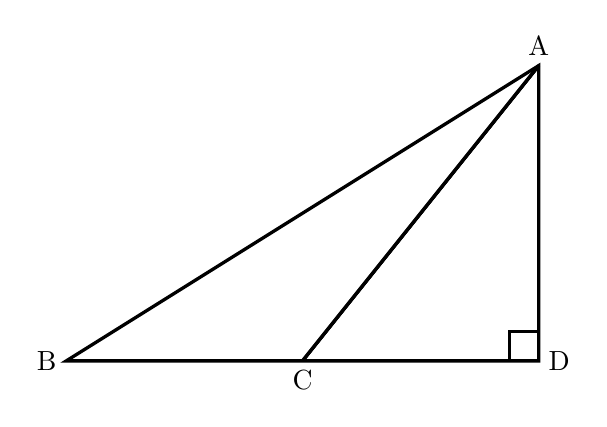
\begin{tikzpicture}[scale=1.5]

% Define vertices
\coordinate (B) at (0,0);
\coordinate (C) at (2,0);
\coordinate (A) at (4,2.5);
\coordinate (D) at (4,0);

% Draw triangle ABD
\draw[very thick] (B) -- (A) -- (D) -- (B) -- cycle;
\draw[very thick] (A) -- (C);

% Draw altitude AC (from A perpendicular to BD)
\draw[very thick] (A) -- (C);

% Draw right angle mark at C
\draw[very thick] (D) ++(0,0.25) -- ++(-0.25,0) -- ++(0,-0.25);

% Vertex labels
\node[above] at (A) {A};
\node[left] at (B) {B};
\node[below] at (C) {C};
\node[right] at (D) {D};

\end{tikzpicture}
\end{document}